\section{Экспериментальное исследование}
\label{sec:testing}

\subsection{Тестовое окружение}

В качестве основной конкретной реализации \ukanren для тестирования
использовался OCanren\footnote{Проект OCanren: \url{https://github.com/JetBrains-Research/OCanren}, дата последнего посещения: 15.05.2020}\cite{ocanren},
реализованный на OCaml\cite{ocanren}.
%Для некоторых тестов для использовался faster-miniKanren\footnote{\url{https://github.com/miniKanren/faster-miniKanren}},
%версия miniKanren, реализованная на Scheme.

Тесты запускались на ноутбуке со следующими характеристиками: Intel Core i5-6200U CPU, 2.30GHz, DDR4, 12GiB.

Для тестирования суперкомпилятора и его модификаций использовался следующий алгоритм.
\begin{enumerate}
\item Подготавливается программа, реализованная на внутреннем представлении $\mu$Kanren.
\item Программа и запрос, на который будет происходить специализация, подаются на вход суперкомпилятору.
\item По дереву процессов, порождённому суперкомпилятором, строится остаточная программа.
\item Остаточная программа транслируется в OCanren и
      запускается в заранее подготовленном окружении с тестовыми запросами.
\end{enumerate}


Реализованный суперкомпилятор сравнивался с реализацией \forcpd для $\mu$Kanren\footnote{Проект: \url{https://github.com/kajigor/uKanren_transformations}, дата последнего посещения: 15.05.2020},
а также c реализацией \forcpd для Prolog --- системой ECCE\footnote{Проект ECCE: \url{https://github.com/leuschel/ecce}, дата последнего посещения: 15.05.2020}.
Другие специализаторы не рассматриваются, так как согласно работе~\cite{controlPoly}, специализация с
помощью \forcpd в ECCE показывает лучшие результаты.

Для использования последнего требовалось оттранслировать программу на \ukanren в Prolog, специализировать
её на запрос, далее оттранслировать результирующую программу в OCanren.
Это допустимо сделать в силу того, что между \ukanren и чистым подмножеством Prolog есть
взаимно однозначное синтаксическое соответствие.
Все необходимые средства для этого также предоставлялись указанной библиотекой специализации.


\subsubsection{Набор тестов}

Был выбран следующий набор тестов для тестирования и анализа суперкомпилятора и его модификаций.
\begin{itemize}
 \item Программа \lstinline{doubleAppend(xs, ys, zs, rs)}, которая
       производит конкатенацию трёх списков. Она классически используется
       для проверки эффекта дефорестации в специализированной программе.
       Специализация происходила на запрос \lstinline{doubleAppend} со свободными переменными.
 \item Программа \lstinline{maxLength(xs, max, len)}, которая находит в списке
       максимальный элемент и длину списка. Она классически используется
       для проверки эффекта таплинга в специализированной программе.
       Специализация происходила на запрос \lstinline{maxLength} со свободными переменными.
 \item Программа сортировки \lstinline{sort(list, result)}. Выбрана в силу показательности
       результатов.
       Специализация происходила на запрос \lstinline{sort} со свободными переменными.
%     Запросы:
%     \begin{itemize}
%     \item оптимизация сортировки: \relo{sort}(xs, ys);
%     \item генерация отсортированных последовательностей: \relo{sort}(xs, xs).
%     \end{itemize}
 \item Отношение, проверяющее принадлежность пути графу \\
       \lstinline{isPath(path, graph, result)}.
       Специализация происходила на запрос \lstinline{isPath(path, graph, True)}.
       Запросы к программе для тестирования:
       \begin{itemize}
       \item поиск пути заданного размера в случайном графе: \\
       \lstinline{isPath(path, graph, True)$\land$length(path, N)};
       \item поиск фиксированного количества путей, принадлежащих данному графу.
       %\\ $\text{isPath}^o_s$(p, g)$\land$\relo{length}(p, N).
       \end{itemize}

	   В приложении А на рисунке~\ref{fig:graphGen} представлен код, который
	   был использован для генерации графов. Функции на вход
	   подаётся количество вершин, количество рёбер и зерно для генератора случайных чисел.
	   В тестах приводятся три графа на 20 вершинах с 50 рёбрами
	   с зёрнами: граф 1 --- 42, граф 2 --- 34, граф 3 --- 106.

 \item Интерпретатор формул логики высказываний \\ \lstinline{logint(formula, subst, result)}.
       Интерпретатор специализируется на то, чтобы всегда генерировать выполнимые формулы
       \lstinline{logint(formula, subst, True)}.
%      Запросы:
%     \begin{itemize}
%     \item поиск $n$ решений заданной формулы;
%     \item генерация $n$ формул с подстановке размера $n$.
%     \end{itemize}
 \item Интерпретатор лямбда-исчисления \lstinline{lam(expr, result)}.
       Интерпретатор специализируется на выражение \lstinline{lam(expr, result)}
       и используется для генерации $n$ выражений в нормальной форме \lstinline{lam(expr, expr)};
 	%\item генерация $n$ выражений, редуцирующихся к заданному выражению \lstinline{lam(expr, E)}.
 \item Проверка типов в просто типизировнном лямбда-исчислении \lstinline{infer(typ, expr)}.
%   \begin{itemize}
% 	\item Поиск $n$ обителей заданного типа.
% 	\item
     Отношение использовалось для генерация выражений, соответствующих заданной спецификации типа и выржения.
     Специализируется выражение:\\
 	 %\relo{infer}(type, expr) $\land$ type $\equiv$ TYPE\_SPEC $\land$ expr $\equiv$ EXPR\_SPEC.
 	 \lstinline{infer(typ, expr)$\land$typ $\equiv$ TYPE_SPEC$\land$expr $\equiv$ EXPR_SPEC}
 %  \end{itemize}
% \item Интерпретатор простого подмножества Scheme.
%    \begin{itemize}
%    \item \todo{Интересный тест!}
%    \end{itemize}
\end{itemize}

% Все вышеперечисленные программы были применены к реализованным суперкомпиляторами,
Ко всем вышеперечисленным программам были применены суперкомпиляторы,
и результаты выполнения остаточных программ были проверены на адекватность и соответствие задачам исходных программ.
Проводилось 10 измерений, пока которым выводились средние значения.
Следует отметить, что задачи доказательства сохранения семантики суперкомпилятором на стояло.

\subsection{Пример работы базового суперкомпилятора \ukanren}
% Для начала разберём, как базовый суперкомпилятор ведёт себя на
% базовом наборе программ, результат которых несложно проанализировать.

% \begin{itemize}
% \item Классическая программа \lstinline{doubleAppend}~\cite{cpd}, которая используется для
%       проверки наличия эффекта дефорестации (\todo{В приложении}).
% %\item Другая классическая программа \lstinline{maxLength}~\cite{cpd}, которая
% %      используется для проверки наличия эффекта таплинга.
% \end{itemize}

Разберём на примере результат работы базового суперкомпилятора.

Классическая программа для тестирования эффектов специализации ---
\lstinline{doubleAppend}, представленная на рисунке~\ref{fig:dappCode},
в которой происходит конкатенация списков трёх списков.

\begin{figure}[h!]
\begin{lstlisting}
doubleAppend a b c d =
  fresh (t)
   (append a b t $\land$ append t c d)
append y4 y5 y6 =
  (y4 $\equiv$ [] $\land$ y6 $\equiv$ y5) $\lor$
  fresh (ty t h)
   (y4 $\equiv$ h :: t $\land$
    y6 $\equiv$ h :: ty $\land$
    append t y5 ty)
\end{lstlisting}
\caption{Программа для тестирования \lstinline{doubleAppend}}
\label{fig:dappCode}
\end{figure}

Во многих бенчмарках~\cite{cpdPract, controlPoly} это программа используется
для проверки эффекта дефорестации.

Рассмотрим дерево процессов на рисунке~\ref{fig:dappTree}
(для компактности \lstinline{append} сокращён до \lstinline{app}),
которое порождается применением базового
суперкомпилятора к программе \lstinline{doubleAppend}, причём в
качестве аргументов --- простые свободные переменные, из-за чего
просто оптимизируется сама структура программы.

\begin{figure}[h!]
\center
\begin{minipage}[h]{\textwidth}
  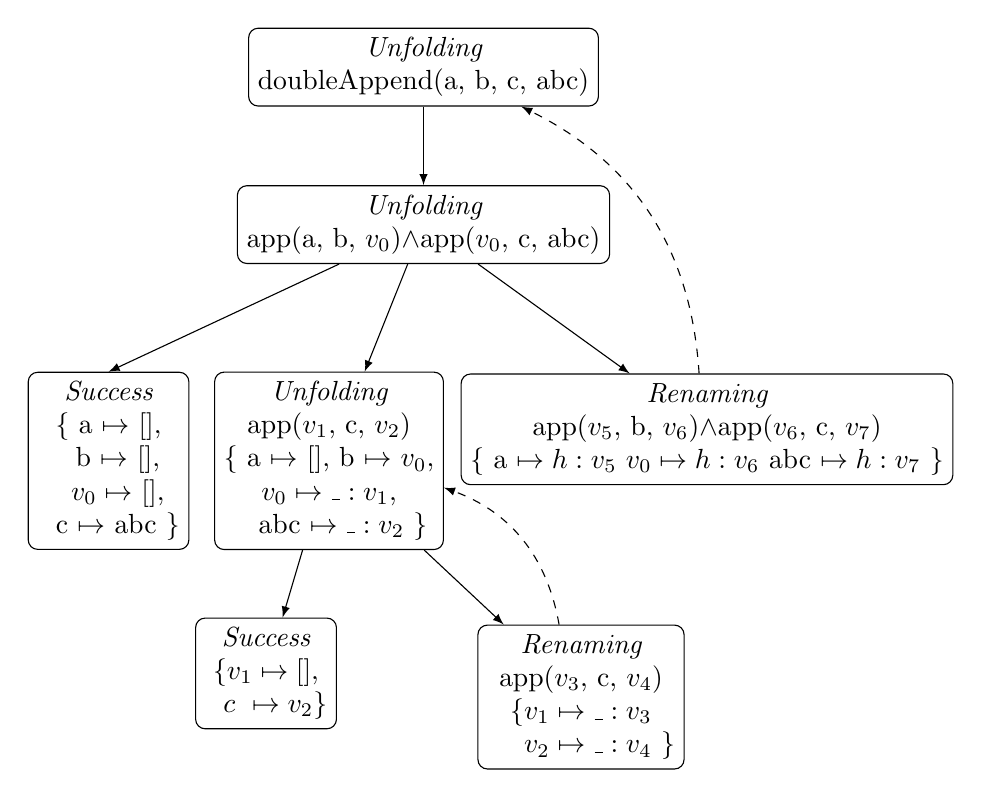
\begin{tikzpicture}[->,node distance=3cm, sibling distance=5cm, level distance=2cm]
    \tikzstyle{conf}=[rectangle,draw, rounded corners=.8ex,align=center]
    \node[conf] (root)   at (0, 0)     {{\it Unfolding} \\ \lstinline{doubleAppend(a, b, c, abc)}};
    \node[conf] (appapp) at (0, -2)    {{\it Unfolding} \\ \lstinline{app(a, b, $\text{v}_0$)$\land$app($\text{v}_0$, c, abc)}};
    \node[conf] (app1)   at (-1.2, -5) {{\it Unfolding} \\ \lstinline{app($\text{v}_1$, c, $\text{v}_2$)} \\ $\{$ a $\mapsto$ [], b $\mapsto$ $\text{v}_0$, \\ $\text{v}_0 \mapsto \_ : \text{v}_1$, \\ $\ \ $ abc $\mapsto \_ : \text{v}_2$ $\}$};
    \node[conf] (app2)   at (3.6, -4.6) {{\it Renaming} \\ \lstinline{app($\text{v}_5$, b, $\text{v}_6$)$\land$app($\text{v}_6$, c, $\text{v}_7$)} \\ $\{$ a $\mapsto \text{h} : \text{v}_5$  $\text{v}_0 \mapsto \text{h} : \text{v}_6 $  abc $\mapsto \text{h} : \text{v}_7$  $\}$};
    \node[conf] (appS)   at (-4,-5)    {{\it Success} \\ $\{$ a $\mapsto$ [], \\ \ \ b $\mapsto$ [],\\ \ \ $\text{v}_0 \mapsto$ [], \\ \ \ c $\mapsto$ abc $\}$};
    \node[conf] (app11)  at (2,  -8)  {{\it Renaming} \\ \lstinline{app($\text{v}_3$, c, $\text{v}_4$)} \\ $\{\text{v}_1 \mapsto \_ : \text{v}_3 $ \\ $\ \ \ \ \text{v}_2 \mapsto \_ : \text{v}_4 $  $\}$};
    \node[conf] (app1S)  at (-2, -7.7) {{\it Success} \\ $\{ \text{v}_1 \mapsto [],$ \\ $\ \ c \ \mapsto \text{v}_2 \}$};
    \draw[-latex] (root) -- (appapp);
    \draw[-latex] (appapp) -- (appS.north);
    \draw[-latex] (appapp) -- (app1);
    \draw[-latex] (appapp) -- (app2);
    \draw[-latex] (app1) -- (app1S);
    \draw[-latex] (app1) -- (app11);
    \draw[-latex,dashed] (app2) edge [bend right] (root);
    \draw[-latex,dashed] (app11) edge [bend right] (app1);
  \end{tikzpicture}
\end{minipage}
\caption{Дерево процессов для программы \lstinline{doubleAppend}}
\label{fig:dappTree}
\end{figure}

В приведённом дереве первым этапом происходит замена определения \lstinline{doubleAppend}
на его тело. Так как в определении нет дизъюнкий, получаем всего одну конфигурацию,
в которой операцией \lstinline{fresh} добавляется новая семантическая переменная $\texttt{v}_0$.
Далее происходит обработка конфигурации с более чем одним конъюнктом. Так как используется
полная стратегия развёртывания, каждая из конъюнкий раскрывается по определению и
рассматривается их дизъюнктивная нормальная форма, в которой всего четыре дизъюнкта,
один из которых не унифицируется, поэтому всего появляется только три конфигурации.
Эти конфигурации рассматривают несколько возможных значений переменных:
\begin{enumerate}
\item когда \lstinline{a} и \lstinline{b} пустые списки, то результатом конкатенации
является \lstinline{c};
\item если же \lstinline{b} не пуст, тогда результат --- это конкатенация списков \lstinline{b} и \lstinline{c}.
      Отношение конкатенации двух списков также специализируется под задачу.
      В результате этой специализации порождается исходное отношение, поскольку
      никакой новой информации не было выявлено и исходная программа уже была оптимальна;
\item в третьем же случае выводится, что результат конкатенации трёх списков
      \lstinline{a}, \lstinline{b} и \lstinline{c} --- это конкатенация
      списков $\texttt{v}_5$, \lstinline{b} и \lstinline{c}, где $\texttt{v}_5$
      является хвостом списка, а в голову которой добавили голову \lstinline{a}.
\end{enumerate}

По данному дереву порождается остаточная программа, изображённая на рисунке~\ref{fig:dappCodeOpt}.
\begin{figure}[h!]
\begin{lstlisting}
doubleAppendo a b c d =
  fresh (x4) (app3 a b x4 c d)
app3 a b t c d =
   fresh (x7 x6 x5 x10 x9 x8)
     (a $\equiv$ [] $\land$ b $\equiv$ t $\land$
       (t $\equiv$ [] $\land$ c $\equiv$ d $\lor$
       (t $\equiv$ x8 :: x9) $\land$
        d $\equiv$ x8 :: x10 $\land$
        app2 x9 c x10
     ) $\lor$
     (a $\equiv$ x5 :: x6 $\land$
      t $\equiv$ x5 :: x7 $\land$
      d $\equiv$ x5 :: x10 $\land$
      app3 x6 b x7 c x10) )
app2 a b c =
  fresh (x13 x12 x11)
   (a $\equiv$ [] $\land$ b $\equiv$ c $\lor$
   (a $\equiv$ x11 :: x12 $\land$
    c $\equiv$ x11 :: x13 $\land$
    app x12 b x13))
\end{lstlisting}
\caption{Суперкомпилированная программа \lstinline{doubleAppend}}
\label{fig:dappCodeOpt}
\end{figure}

В итоге, наблюдается, как двупроходный алгоритм становится однопроходным.


\subsection{Сравнение вариаций суперкомпилятора \ukanren}

В таблицах используются условные обозначения для стратегий развёртывания:
\begin{itemize}
\item {\it Full} и {\it Full-non-rec} обозначают полную стратегию и полную стратегию развёртывания с приоритетом на нерекурсивные вызовы соответственно;
\item {\it Seq} обозначает последовательную стратегию развёртывания;
\item {\it Non-rec} и {\it Rec} обозначают нерекурсивную и рекурсивную стратегии соответственно;
\item {\it Min} и {\it Max} обозначают минимальную и максимальную стратегии соответственно;
\item {\it First} обозначает стратегию, при которой всегда развёртывается первый конъюнкт.
\end{itemize}

А также для суперкомпиляторов:
\begin{itemize}
\item {\it Б.С.} обозначает базовый суперкомпилятор с обобщением вниз на предков;
\item {\it М.1 } обозначает модификацию, при которой происходит запрет на обобщение сразу после обобщения;
\item {\it M.2 } обозначает модификацию, при которой обобщение происходит на все ранее вычисленные вершины;
\item {\it M.3 } обозначает модификацию, при которой происходит обобщение вверх на родительские вершины;
\item {\it M.4 } обозначает модификацию, при которой происходит обобщение вверх на родительские вершины, кроме корневой.
\item {\it M.5 } обозначает модификацию, при которой происходит обобщение вверх на родительские вершины, а также запрет обобщения после обобщения.
\end{itemize}


В таблице~\ref{fig:dappTest} представлены результаты сравнения модификаций
с базовым суперкомпилятором при разных стратегиях развёртывания.
При полных стратегиях для \lstinline{doubleAppend} возникает эффект дефорестации.
В остальных стратегиях этого не происходит, из-за чего исполнения по
крайней мере в два раза хуже. Из-за того, что программа довольно небольшая,
модификации алгоритма суперкомпиляции хотя не и оказывают влияния, результат не ухудшают.

\begin{table}[h!]
\center
\begin{tabular}{|l|c|c|c|c|c|c|}
\hline
                   &{\it Б.С.}&{\it М.1}&{\it М.2}&{\it М.3}&{\it M.4} & {\it M.5} \\ \hline
%Original: 0.010374
%ECCE: 0.004058
%CPD: 0.012664
{\it Full        }& {\bf 0.0049}  & 0.0055       & 0.0056       & {\bf 0.0050} & {\bf 0.0048} & 0.0053\\ \hline
{\it Full-non-rec}& 0.0053        & {\bf 0.0048} & {\bf 0.0049} & {\bf 0.0050} & {\bf 0.0037} & {\bf 0.0039} \\ \hline
{\it Seq         }& 0.0098        & 0.0119       & 0.0099       & 0.0127       & 0.0097       & 0.0102 \\ \hline
{\it Non-rec     }& 0.0100        & 0.0122       & 0.0099       & 0.0099       & 0.0097       & 0.0098 \\ \hline
{\it Rec         }& 0.0094        & 0.0133       & 0.0103       & 0.0098       & 0.0097       & 0.0100 \\ \hline
{\it Min         }& 0.0096        & 0.0122       & 0.0100       & 0.0093       & 0.0094       & 0.0099 \\ \hline
{\it Max         }& 0.0096        & 0.0096       & 0.0092       & 0.0101       & 0.0119       & 0.0091 \\ \hline
{\it First       }& 0.0120        & 0.0094       & 0.0094       & 0.0099       & 0.0093       & 0.0093 \\ \hline

\end{tabular}
\caption{Результат для \lstinline{doubleAppendo} c конкатенацией трёх списков длины 120, секунды}
\label{fig:dappTest}
\end{table}

В таблице~\ref{fig:maxlenTest} указаны результаты выполнения для
программы \lstinline{maxLength} на списке \lstinline{[1..200]}.

\begin{table}[h!]
\center
\begin{tabular}{|l|c|c|c|c|c|c|}
\hline
                  &{\it Б.С.}   &{\it М.1}      &{\it М.2}      &{\it М.3}&{\it M.4} & {\it M.5}\\ \hline
%Orig: 0.270905
%ECCE: 0.230436
%CPD: 0.653551
{\it Full        } & 0.623        & 0.638       & {\bf 0.250}  & {\bf 0.250} & {\bf 0.251} & 0.293 \\ \hline
{\it Full-non-rec} & 0.633        & 0.611       & 0.602        & 0.256       & 0.258 & 0.298 \\ \hline
{\it Seq         } & 0.285        & 0.290       & 0.289        & 0.289       & 0.287 & 0.286 \\ \hline
{\it Non-rec     } & 0.284        & 0.289       & 0.285        & 0.285       & 0.287 & 0.287 \\ \hline
{\it Rec         } & 0.856        & 0.893       & 0.560        & 0.577       & 0.569 & 0.888 \\ \hline
{\it Min         } & 0.317        & {\bf 0.280} & 0.303        & 0.284       & 0.279 & {\bf 0.280} \\ \hline
{\it Max         } & {\bf 0.279}  & 0.287       & 0.279        & 0.278       & 0.284 & 0.281 \\ \hline
{\it First       } & 0.864        & 0.858       & 0.564        & 0.963       & 0.949 & 0.565 \\ \hline


\end{tabular}
\caption{Запуск для \lstinline{maxLength} на списке \lstinline{[1..200]}, секунды}
\label{fig:maxlenTest}
\end{table}

Модификация алгоритма {\it M.2-M.4} на стратегии {\it Full} породили программы
с эффектов таплинга, при котором максимальный элемент и длина списка высчитывались
за один проход. Интересное наблюдение состоит в том, что в других случаях, к примеру,
при применении стратегии {\it Seq}, таплинга не происходит, но сама программа
исполняется не существенно медленнее.

В таблице~\ref{fig:sortTest} указаны результаты тестирования для
программы \lstinline{sort} при сортировки списков случайного содержания (числа от 0 до 50)
длины 50.

\begin{table}[h!]

\center
\begin{tabular}{|l|c|c|c|c|c|c|}
\hline
                  &{\it Б.С.}&{\it М.1}&{\it М.2}&{\it М.3}&{\it M.4}&{\it M.5}\\ \hline
{\it Full        } & {\bf 0.239} & 0.252       & {\bf 0.238} & {\bf 0.232} & {\bf 0.239} & 0.244 \\ \hline
{\it Full-non-rec} & 0.241       & {\bf 0.240} & 0.241       & 0.241       & 0.245       & {\bf 0.242} \\ \hline
{\it Seq         } & 0.242       & {\bf 0.240} & {\bf 0.239} & 0.238       & {\bf 0.240} & 0.254 \\ \hline
{\it Non-rec     } & 0.245       &  0.242      & 0.247       & {\bf 0.236} & 0.244       & {\bf 0.242} \\ \hline
{\it Rec         } & 0.239       &  0.242      & 0.252       & 0.240       & 0.250       & 0.243 \\ \hline
{\it Min         } & 0.245       & 0.252       & 0.242       & 0.242       & 0.292       & 0.279 \\ \hline
{\it Max         } & 0.246       & 0.242       & 0.249       & 0.246       & 0.246       & 0.239 \\ \hline
{\it First       } & 0.250       & 0.248       & 0.263       & 0.245       & 0.239       & 0.247 \\ \hline


\end{tabular}
\caption{Запуск для \lstinline{sort}, секунды}
\label{fig:sortTest}
\end{table}

Примечательно, что на всех списках указанного свойства алгоритмы отработали практически
одинаково. Более примечательно, что какие бы модификации ни взяли,
порождаются довольно схожие программы. Это обосновывается тем, что само отношение
сортировки имеет весьма короткое рекурсивное определение.

В таблицах~\ref{fig:logintTest1},~\ref{fig:logintTest2} и~\ref{fig:logintTest3} указаны результаты тестирования для
программы \lstinline{logint}, которая использовалась для генерации всех выполнимых формул
без свободных переменных, с одной свободной переменной и с двумя свободными переменными соответственно.

\begin{table}[h!]
\center
\begin{tabular}{|l|c|c|c|c|c|c|}
\hline
   &{\it Б.С.}&{\it М.1}&{\it М.2}&{\it М.3}&{\it M.4}&{\it M.5}\\ \hline
{\it Full        } &    -        &    -         & 0.132       &  0.105       &    -        & -     \\ \hline
{\it Full-non-rec} & {\bf 0.076} & 0.072        & 0.210       &  0.111       & 0.126       & {\bf 0.081} \\ \hline
{\it Seq         } & 0.168       & 0.181        & 0.149       &  0.090       & {\bf 0.091} & 0.113 \\ \hline
{\it Non-rec     } & 0.078       & 0.092        & 0.136       &  0.088       & 0.114       & 0.099 \\ \hline
{\it Rec         } & 0.081       & 0.074        & {\bf 0.095} &  {\bf 0.064} & 0.126       & 0.090 \\ \hline
{\it Min         } & 0.080       & {\bf 0.064}  & 0.110       &  0.092       & 0.117       & 0.082 \\ \hline
{\it Max         } & 0.164       & 0.193        & 0.144       &  0.077       & 0.111       & 0.146 \\ \hline
{\it First       } & 0.181       & 0.164        & 0.176       &  0.070       & 0.189       & 0.136 \\ \hline
\end{tabular}
\caption{Запуск \lstinline{logint} для генерации формул без переменных, секунды.}
\label{fig:logintTest1}
\end{table}

\begin{table}[h!]
\center
\begin{tabular}{|l|c|c|c|c|c|c|}
\hline
   &{\it Б.С.}&{\it М.1}&{\it М.2}&{\it М.3}&{\it M.4}&{\it M.5} \\ \hline
{\it Full        }&    -         &     -        & 0.078       & 0.068       &    -        &  -  \\ \hline
{\it Full-non-rec}& 0.056        &  0.045       & 0.125       & 0.084       & 0.082       & 0.051\\ \hline
{\it Seq         }& 0.109        &  0.110       & 0.086       & 0.063       & 0.074       & 0.069 \\ \hline
{\it Non-rec     }& {\bf 0.046}  &  {\bf 0.038} & 0.081       & 0.072       & {\bf 0.067} & {\bf 0.045} \\ \hline
{\it Rec         }& 0.055        &  0.050       & 0.074       & {\bf 0.055} & 0.079       & 0.055\\ \hline
{\it Min         }& 0.053        &  0.041       & {\bf 0.066} & {\bf 0.055} & 0.079       & 0.059\\ \hline
{\it Max         }& 0.100        &  0.117       & 0.108       & 0.057       & 0.074       & 0.077\\ \hline
{\it First       }& 0.118        &  0.103       & 0.091       & 0.068       & 0.101       & 0.084\\ \hline
\end{tabular}
\caption{Запуск \lstinline{logint} для генерации формул с одной переменной, секунды.}
\label{fig:logintTest2}
\end{table}

\begin{table}[h!]
\center
\begin{tabular}{|l|c|c|c|c|c|c|}
\hline
   &{\it Б.С.}&{\it М.1}&{\it М.2}&{\it М.3}&{\it M.4}&{\it M.5} \\ \hline
{\it Full        }&    -        &    -        & 0.078       & 0.062      &    -        & - \\ \hline
{\it Full-non-rec}& 0.137       & 0.040       & 0.093       & 0.042      & 0.069       & {\bf 0.040} \\ \hline
{\it Seq         }& 0.086       & 0.082       & 0.066       & 0.049      & {\bf 0.050} & {\bf 0.041} \\ \hline
{\it Non-rec     }& 0.043       & {\bf 0.031} & 0.063       & 0.044      & 0.055       & 0.046 \\ \hline
{\it Rec         }& {\bf 0.037} & 0.034       & {\bf 0.045} & 0.040      & 0.051       & 0.049 \\ \hline
{\it Min         }& {\bf 0.037} & 0.039       & 0.049       & 0.041      & 0.054       & 0.045 \\ \hline
{\it Max         }& 0.068       & 0.070       & 0.067       &{\bf 0.036} & 0.062       & 0.071 \\ \hline
{\it First       }& 0.104       & 0.100       & 0.110       & 0.095      & 0.137       & 0.073 \\ \hline
\end{tabular}
\caption{Запуск \lstinline{logint} для генерации формул с двумя переменными, секунды.}
\label{fig:logintTest3}
\end{table}

Прочерки в таблицах обозначают то, что из-за большой требовательности к ресурсам,
на тех модификациях, которые не приводят к быстрому сворачиванию программ,
включая и базовый суперкомпилятор, не удалось получить оптимизированные программы.
Однако ожидается,
что при должном количестве ресурсов порождённые программы окажутся слишком большими,
что приведёт к значительным проблемам производительности, из-за чего добиваться
результатов
для данных случаев в данной работе считается нецелесообразным.

В представленных таблицах наблюдается, что при увеличении количества свободных переменных,
в среднем, уменьшается время генерации формул. Это обосновывается тем, что в
деревьях исполнения порождаемых программам больше ветвей оканчиваются успешным
поиском значения в подстановке.



\subsubsection{Исследование модификации с ограничением неэквивалентности}

Для исследования влияния ограничения неэквивалентности рассматривается отношение
интерпретатора лямбда-исчисления \lstinline{lam}, с помощью которого
происходил поиск 50-ти термов в нормальной форме.

В таблице~\ref{fig:lamTestSimple} приведено время выполнения программы
без введения ограничения неэквивалентности. Здесь наблюдается интересная закономерность:
на очередном интерпретаторе модификации {\it M.1} и {\it M.5} показывают лучшие результаты.

\begin{table}[h!]
\center
\begin{tabular}{|l|c|c|c|c|c|c|}
\hline
   &{\it Б.С.}&{\it М.1}&{\it М.2}&{\it М.3}&{\it M.4}&{\it M.5} \\ \hline

{\it Full        } & {\bf 0.106}& 0.088     & 0.102       & 0.106       & 0.095       & 0.084 \\ \hline
{\it Full-non-rec} & {\bf 0.106}& 0.086     & 0.111       & 0.105       & {\bf 0.083} & 0.082 \\ \hline
{\it Seq         } & 0.107      & 0.085     & 0.105       & {\bf 0.103} & {\bf 0.083} & {\bf 0.080} \\ \hline
{\it Non-rec     } & 0.112      & 0.087     & 0.{\bf 100} & 0.110       & 0.086       & 0.084 \\ \hline
{\it Rec         } & 0.111      &{\bf 0.083}& 0.112       & 0.111       & 0.090       & 0.083 \\ \hline
{\it Min         } & 0.109      & 0.095     & 0.110       & 0.114       & 0.093       & 0.085 \\ \hline
{\it Max         } & 0.107      & 0.098     & 0.105       & 0.105       & 0.086       & 0.086 \\ \hline
{\it First       } & {\bf 0.106}& 0.089     & 0.111       & 0.118       & 0.093       & 0.092 \\ \hline
\end{tabular}
\caption{Запуск \lstinline{lam} для поиска термов в нормальной форме без оператора неэквивалентности, секунды.}
\label{fig:lamTestSimple}
\end{table}

В таблице~\ref{fig:lamTestDiseqSimple} указано время исполнения на программе с
использованием оператора неэквивалентности только в отношении подстановки, которое
используется интерпретатором.

\begin{table}[h!]
\center
\begin{tabular}{|l|c|c|c|c|c|c|}
\hline
   &{\it Б.С.}&{\it М.1}&{\it М.2}&{\it М.3}&{\it M.4}&{\it M.5} \\ \hline

{\it Full        } & {\bf 0.040} &  0.025    & 0.052     &0.046      & 0.024     & 0.024 \\ \hline
{\it Full-non-rec} & 0.042       &  0.025    & 0.042     &0.044      & 0.024     & 0.025 \\ \hline
{\it Seq         } & 0.044       &  0.026    & 0.046     &0.045      &{\bf 0.022}& 0.027 \\ \hline
{\it Non-rec     } & {\bf 0.040} &  0.026    & 0.046     &0.042      & 0.025     &{\bf 0.022} \\ \hline
{\it Rec         } & 0.045       &{\bf 0.023}&{\bf 0.041}&0.044      & 0.027     &{\bf 0.022} \\ \hline
{\it Min         } & 0.042       &  0.034    & 0.045     &0.045      & 0.023     & 0.027 \\ \hline
{\it Max         } & 0.043       &  0.026    & 0.043     &{\bf 0.040}& 0.027     & 0.028 \\ \hline
{\it First       } & 0.044       &  0.027    & 0.045     &0.042      & 0.025     & 0.023 \\ \hline
\end{tabular}
\caption{Запуск \lstinline{lam} для поиска термов в нормальной форме с оператором неэквивалентности, секунды.}
\label{fig:lamTestDiseqSimple}
\end{table}

Из таблицы виден прирост производительности для методов {\it М.1}, {\it M.4} и
{\it M.5} практически в четыре раза, а для остальных -- в два. \\

% Однако оператор можно использовать и для реализации самого интерпретатора при
% определении, является ли левая часть аппликации лямбда-теромом.
%
% \begin{table}[h!]
% \center
% \begin{tabular}{|l|c|c|c|c|c|c|}
% \hline
%                   &{\it Б.С.}  &{\it М.1}  &{\it М.2}  &{\it М.3}  &{\it M.4}  &{\it M.5} \\ \hline
% {\it Full        }&0.050       &  0.042    & 0.052     & 0.048     & 0.037     & 0.041 \\ \hline
% {\it Full-non-rec}&0.048       &  0.048    & 0.050     & 0.047     & 0.038     & 0.041 \\ \hline
% {\it Seq         }&{\bf 0.046} &{\bf 0.036}& 0.048     &{\bf 0.046}& 0.039     & 0.038 \\ \hline
% {\it Non-rec     }&0.049       &  0.041    & 0.049     & 0.049     & 0.042     &{\bf 0.036} \\ \hline
% {\it Rec         }&0.049       &  0.042    & 0.050     & 0.048     & 0.041     &{\bf 0.036} \\ \hline
% {\it Min         }&{\bf 0.046} &  0.040    & 0.045     & 0.047     & 0.037     & 0.037 \\ \hline
% {\it Max         }&0.051       &  0.038    &{\bf 0.044}& 0.048     &{\bf 0.036}& 0.042 \\ \hline
% {\it First       }&0.049       &  0.044    & 0.049     & 0.049     & 0.042     & 0.041 \\ \hline
% \end{tabular}
% \caption{Запуск \lstinline{lam} для поиска термов в нормальной форме c оператором неэквивалентности, секунды.}
% \label{fig:lamTestDiseq}
% \end{table}

% Несмотря на то, что разные подходы на разных классах программ показывают
% себя с лучшей стороны, в среднем модификация с обобщением вверх при
% нерекурсивной стратегии развёртывания показывает себя лучше всего.

Разные подходы показывают себя хорошо на разных классах задач.
При этом стабильно самой неудачной стратегией развёртки себя
показывает стратегия {\it First}. Самыми неудачными модификациями оказались
{\it M.1} и {\it М.2}.
Модификация \textit{M.2} с обобщением на все рассмотренные вершины стабильно приводит
к слишком раннему сворачиванию дерева, из-за чего теряется точность специализации.
Модификация \textit{M.1}, наоборот, делает слишком много развёртываний, что также
приводит к потере производительности.
В целом, смена стратегии базового суперкомпилятора позволила увеличить
производительность большинства порождаемых программ. В среднем, лучше
всего работают стратегии \textit{Seq} и её модификация \textit{Non-rec}.
Реализация обобщения вверх \textit{M.3} значительно улучшила производительность программ.
Её модификация \textit{M.4} выигрывала в больших случаях, однако периодически
значительно проигрывает, как и модификация \textit{M.5}, которая хорошо показала
себя только на интерпретаторах.

В итоге, оптимальной модификацией считается суперкомпилятор с обобщением
вверх с нерекурсивной стратегией развёртывания.


\subsection{Сравнение суперкомпилятора с существующими решениями}

В таблице~\ref{fig:totalResult} представлены результаты сравнения базового алгоритма
суперкомпиляции ({\it Б.С,}) и выбранной наиболее успешной модификации
суперкомпилятора ({\it М.С.}) с оригинальными программами ({\it Оригинал}),
а также с оптимизированными программами с помощью
системы ECCE для Prolog с использованием трансляции ({\it ECCE}) и адаптации
конъюнктивной частичной дедукции для miniKanren ({\it CPD}).

\begin{table}[h!]
\center
\begin{tabular}{|c|c|c|c|c|c|}
\hline
{\it Параметр} & {\it Оригинал} & {\it ECCE }  & {\it CPD} & {\bf Б.C} & {\bf М.С.} \\ \hline
{\bf doubleAppend} & \multicolumn{5}{|l|}{списки фиксированной длины } \\ \hline
120                & 0.0135 & 0.0051 & 0.0133 & {\bf 0.0049} & 0.0098 \\ \hline


{\bf maxLength} & \multicolumn{5}{|l|}{фиксированный список} \\ \hline

       [1..200] & 0.257 & {\bf 0.230} & 0.727 & 0.623 & 0.287 \\ \hline


%\rowcolor{black!10}
{\bf sort} & \multicolumn{5}{|l|}{случайный список фиксированной длины } \\ \hline
50       & 8.42     & 12.28 & 13.2 & 0.239  & {\bf 0.242} \\ \hline

%\rowcolor{black!10}
 {\bf isPath} & \multicolumn{5}{|l|}{10 путей} \\ \hline
  граф 3      & > 300 & {\bf 1.03} & 1.19 & 2.43 & 1.81 \\ \hline

 {\bf isPath} & \multicolumn{5}{|l|}{произвольный путь длины 7} \\ \hline
   граф 3     & 62.12 & 1.08 & 1.15 & 1.34 & {\bf 0.85} \\ \hline
 {\bf isPath} & \multicolumn{5}{|l|}{произвольный путь длины 10} \\ \hline
 граф 1  &  12.51  & 1.01 & 1.20 &  1.28 & {\bf 0.48} \\
 граф 2  &  > 300s & 1.73 & 2.09 & 0.85 & {\bf 0.48} \\
 граф 3  &         & 9.90 & 12.73& 3.29 & {\bf 1.23} \\
 \hline

%\rowcolor{black!10}
{\bf logint} & \multicolumn{5}{|l|}{размер подстановки} \\ \hline
0 & > 300    & 0.17  & 2.7  & -  &  {\bf 0.11} \\
1 &          & 0.09  & 1.7  & -  &  {\bf 0.07} \\
2 &          & 0.08   & 0.9  & -  & {\bf 0.05} \\
\hline

%\rowcolor{black!10}
{\bf lam} & \multicolumn{5}{|l|}{термы в нормальной форме} \\ \hline
%10 термов к себе    & 0.17     & 0.001 & 0.008 & 0.002  \\
50 термов & > 300    & 2.98  & 0.08 & 0.08 & {\bf 0.04}   \\
%1000 термов к const & 1.01     & 0.126 & 0.263 & 0.274  \\
\hline
% {\bf scheme} & \multicolumn{5}{|l|}{программы, сводящиеся к const} \\ \hline
% 41 терм      &
{\bf genBySpec} & \multicolumn{5}{|l|}{генерация по спецификации} \\ \hline
2000            & > 300 & 0.53 & 0.62 & - & {\bf 0.36} \\ \hline
\end{tabular}
\caption{Результаты сравнения алгоритмов специализации, cекунды}
\label{fig:totalResult}
\end{table}

В случае с \lstinline{doubleAppend}, которому на вход подали три одинаковых списка длины 120,
базовому суперкомпилятору удалось
добиться эффекта дефорестации и сравниться с {\it ECCE}, модифицированный суперкомпилятор
уступает {\it ECCE}, однако всё ещё быстрее как оригинальной программы, так и {\it CPD}.

Однако в тесте \lstinline{maxLength}, которому на вход подали список [1..200], базовый суперкомпилятор пусть и делает
таплинг, но добавляет ветвистости программе, из-за чего она работает хуже оригинальной
почти в два раза, однако модифицированный алгоритм пусть не ускоряет исполнение программы,
ухудшает её незначительно, в отличие от {\it CPD}. Стоит заметить, что ECCE пусть и
улучшил производительность, отличие от оригинальной программы оказалось несущественным.

Исполнение программы сортировки \lstinline{sort} на случайном списке длины 50 и элементами
не более 50, в свою очередь, заметно ускорилось относительно и оригинала, и специализированных
программ с помощью конъюнктивной частичной дедукции. Это может объясняться тем, что в некоторых
случаях методы конъюнктивной частичной дедукции делают лишние развёртывания, что в конечном
счёте приводит к ухудшению программы.

Отношение проверки принадлежности пути графу \lstinline{isPath} использовалось
для поиска 10 путей в указанном графе. Здесь результат работы суперкомпиляции
проиграл примерно в два раза алгоритмам конъюнктивной частичной дедукции,
но решил задачу значительно быстрее оригинала. Однако уже на более
осмысленной задаче по поиску путей заданной длины суперкомпилятор
значительно выиграл у методов конъюнктивной частичной дедукции.


Также был рассмотрен интерпретатор логических формул \lstinline{logint}, который
запускался для поиска формул и их подстановок, в которой они выполняются, для
формул с нулём, одним и двумя свободными переменными. Это пример запуска в ``обратную''
сторону, который, как можно наблюдать из таблицы, действительно крайней неэффективен.
Специализированные же версии дают значительный прирост производительности, однако
модифицированная версия суперкомпилятора выигрывает у всех методов. Прочерки стоят,
как объяснялось в предыдущем подразделе, из-за того, что в данном случае стратегия
полного развёртывания требовала слишком много ресурсов.

В примере с отношением \lstinline{lam} базовый суперкомпилятор отработал
идентично \textit{CPD}, но модифицированный в два раза быстрее нашёл 50 термов
в нормальной форме.

Довольно сложным примерном для суперкомпилятора оказалось отношение
по генерации термов по спецификации:
\begin{itemize}
\item спецификация терма: \lstinline{app (app _ _) _};
\item спецификация типа: \lstinline{_ $\to$ (_ $\to$ not-arrow _)}.
\end{itemize}

% Полная стратегия развёртки базового компилятора вновь не справилась,
% но модификация значительно выигрывает у оригинала и опять побеждает методы
% конъюнктивной частичной дедукции.
Суперкомпиляция с полной стратегией развертки вновь не уложилась в имеющиеся ограничения
на ресурсы, однако модифицированная версия значительно повышает эффективность программы,
даже относительно \textit{ECCE} и \textit{CPD}.

%По результатам экспериментального исследования можно сделать вывод,
%что разработанный суперкомпилятор в среднем показывает хорошие результаты
%и на большинстве рассмотренных программ даёт значительный прирост производительности,
%как относительно оригинальной программы, так и относительно рассмотренных
%методов специализации.

